\section{\textit{Clustering K-Means}}
\par \textit{Clustering} merupakan salah satu metode Data Mining yang bersifat tanpa arahan \textit{(unsupervised)}. Ada dua jenis data clustering yang sering dipergunakan dalam proses pengelompokan data yaitu \textit{hierarchical} (hirarki) data \textit{clustering} dan \textit{non-hierarchical} (non hirarki) data \textit{clustering. K-Means} merupakan salah satu metode data \textit{clustering} non hirarki yang berusaha mempartisi data yang ada ke dalam bentuk satu atau lebih \textit{cluster}/kelompok. Metode ini mempartisi data ke dalam \textit{cluster}/kelompok sehingga data yang memiliki karakteristik yang sama dikelompokkan ke dalam satu\textit{cluster} yang sama dan data yang mempunyai karakteristik yang berbeda dikelompokkan ke dalam kelompok yang lain. Adapun tujuan dari data \textit{clustering} ini adalah untuk meminimalisasikan \textit{objective function} yang diset dalam proses clustering, yang pada umumnya berusaha meminimalisasikan variasi di dalam suatu \textit{cluster} dan memaksimalisasikan variasi antar \textit{cluster}. Data \textit{clustering} menggunakan metode \textit{K-Means} ini secara umum dilakukan dengan algoritma dasar sebagai berikut \cite{sadewo2017penerapan}
\newpage

\subsection{\textit{Clustering}}
\textit{Clustering} Analisis Pengelompokan / \textit{Clustering} merupakan proses membagi data dalam suatu himpunan ke dalam beberapa kelompok yang kesamaan datanya dalam suatu kelompok lebih besar daripada kesamaan data tersebut dengan data dalam kelompok lain. Potensi \textit{Clustering} adalah dapat digunakan untuk mengetahui struktur dalam data yang dapat dipakai lebih lanjut dalam berbagai aplikasi secara luas seperti klasifikasi, pengolahan gambar, dan pengenalan pola \cite{sadewo2017penerapan}.

\subsection{\textit{K-Means}}
\textit{K-Means} merupakan salah satu metode pengelompokan data non-hierarki (sekatan) yang berusaha mempartisi data yang ada ke dalam bentuk dua atau lebih kelompok. Metode ini mempartisi data ke dalam kelompok sehingga data berkarakteristik sama dimasukkan ke dalam satu kelompok yang sama dan data yang berkarakteristik berbeda dikelompokkan kedalam kelompok yang lain. Adapun tujuan pengelompokkan data ini adalah untuk meminimalkan fungsi objektif yang diatur dalam proses pengelompokan, yang pada umumnya berusaha meminimalkan variasi di dalam suatu kelompok dan memaksimalkan variasi antar kelompok.

\par Data clustering menggunakan metode K-Means ini secara umum dilakukan dengan algoritma dasar sebagai berikut :

\begin{enumerate}
    \item Tentukan jumlah \textit{Cluster}.
    \item Alokasi data ke \textit{Cluster} secara \textit{Random}.
    \item Hitung \textit{Centroid} rata-rata dari data yang ada dari masing-masing \textit{Cluster}.
    \item alokasi masing-masing data ke \textit{centroid}/rata-rata terdekat.
    \item Kembali ke Step 3, apabila masih ada data yang berpindah \textit{cluster} atau apabila perubahan nilai \textit{centroid}, ada yang di atas nilai \textit{threshold} yang ditentukan atau apabila perubahan nilai pada \textit{objective function} yang digunakan di atas nilai \textit{threshold}  yang ditentukan.
\end{enumerate}
\par Dalam tulisan ini beberapa hal terkait dengan metode \textit{K-Means} ini berusaha untuk dijelaskan, termasuk di antaranya beberapa pengembangan yang telah dilakukan terhadap\textit{K-Means}, beberapa permasalahan yang harus diperhitungkan dalam menggunakan metode K\textit{K-Means} dalam pengelompokan data, ulasan mengenai keberadaan \textit{K-Means} di antara metode pengklasifikasian dengan arahan \textit{(supervised)} dan tanpa arahan \textit{(unsupervised)}, ulasan singkat mengenai metode \textit{K-Means} untuk dataset yang mempunyai bentuk khusus dan \textit{mixture modelling}, serta algoritma dari metode-metode pengelompokan yang masih digolongkan sebagai pengembangan metode \textit{K-Means}.

\subsection{Pengalokasian ulang data ke dalam \textit{Cluster}}
\par Metode Pengalokasian Ulang Data ke Dalam Masing-Masing \textit{Cluster} Secara mendasar, ada dua cara pengalokasian data kembali ke dalam masing-masing \textit{cluster} pada saat proses iterasi \textit{cluster}. Kedua cara tersebut adalah pengalokasian dengan cara tegas \textit{(hard)}, dimana data item secara tegas dinyatakan sebagai anggota \textit{cluster} yang satu dan tidak menjadi anggota \textit{cluster}  lainnya, dan dengan cara \textit{cluster}, dimana masing-masing data item diberikan nilai kemungkinan untuk bisa bergabung ke setiap \textit{cluster} yang ada. Kedua cara pengalokasian tersebut diakomodasikan pada metode \textit{K-Means}. Perbedaan di antara kedua metode ini terletak pada asumsi yang dipakai sebagai dasar pengalokasian. \textit{K-Means } Pengalokasian kembali data ke dalam masing-masing \textit{cluster} dalam metode  K-Means didasarkan pada perbandingan jarak antara data dengan centroid setiap \textit{cluster}  yang ada. Data dialokasikan ulang secara tegas ke\textit{cluster} yang mempunyai \textit{centroid} terdekat dengan data tersebut. Pengalokasian ini dapat dirumuskan sebagai berikut \cite{pane2018qualitative}

\begin{figure}[h]
\centering
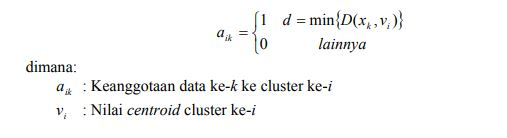
\includegraphics[scale=0.6]{chapters/figures/metclus.JPG}
\caption{Keanggotaan data \textit{Cluster}}
\end{figure}

\subsection{Beberapa permasalahan yang terkait dengan \textit{Clustering K-Means}}
\par Beberapa Permasalahan yang Terkait Dengan \textit{K-Means} Beberapa permasalahan yang sering muncul pada saat menggunakan metode \textit{K-Means} untuk melakukan pengelompokan data adalah: 
\begin{enumerate}
    \item Ditemukannya beberapa model \textit{clustering} yang berbeda 
    \item Pemilihan jumlah \textit{cluster} yang paling tepat 
    \item Bentuk masing-masing \textit{cluster}
    \item . Masalah overlapping Keenam permasalahan ini adalah beberapa hal yang perlu diperhatikan pada saat menggunakan \textit{K-Means} dalam mengelompokkan data. Permasalahan 1 umumnya disebabkan oleh perbedaan proses inisialisasi anggota masing-masing \textit{cluster}. Proses initialisasi yang sering digunakan adalah proses inisialisasi secara \textit{random}. Dalam suatu studi perbandingan, proses inisialisasi secara \textit{random} mempunyai kecenderungan untuk memberikan hasil yang lebih baik dan \textit{independent}, walaupun dari segi kecepatan untuk lebih lambat. Permasalahan 2 merupakan masalah laten dalam metode \textit{K-Means}. Beberapa pendekatan telah digunakan dalam menentukan jumlah \textit{cluster} yang paling tepat untuk suatu dataset yang dianalisa. 
\end{enumerate}
\par Satu hal yang patut diperhatikan mengenai metode-metode ini adalah pendekatan yang digunakan dalam mengembangkan metode-metode tersebut tidak sama dengan pendekatan yang digunakan oleh \textit{K-Means} dalam mempartisi data items ke masing-masing \textit{cluster}. Permasalahan kegagalan untuk converge, secara teori memungkinkan untuk terjadi dalam kedua metode \textit{K-Means} yang dijelaskan di dalam tulisan ini. Kemungkinan ini akan semakin besar terjadi untuk metode  \textit{K-Means}, karena setiap data di dalam dataset dialokasikan secara tegas  untuk menjadi bagian dari suatu \textit{cluster} tertentu. Perpindahan suatu data ke suatu cluster tertentu dapat mengubah karakteristik model \textit{clustering} yang dapat menyebabkan data yang telah dipindahkan tersebut lebih sesuai untuk berada di cluster semula sebelum data tersebut dipindahkan. Demikian juga dengan keadaan sebaliknya. Kejadian seperti ini tentu akan mengakibatkan pemodelan tidak akan berhenti dan kegagalan untuk converge akan terjadi. Untuk suatu \textit{cluster}, walaupun ada, kemungkinan permasalahan ini untuk terjadi sangatlah kecil, karena setiap data diperlengkapi dengan membership \textit{function K-Means} untuk menjadi anggota \textit{cluster} yang ditemukan \cite{setyawan2018comparison}